\section{Short and long response functions}\label{sec:short_long}

Regarding Equation \ref{eq:return_general}, we use a time lag $\tau$ in the
returns to see the gains or loses in a future time. We divide the time lag
$\tau$ as show in Fig. \ref{fig:tau_short_long}. As

\begin{equation}\label{eq:tau_short_long}
    \tau = \tau' + \left( \tau - \tau' \right)
\end{equation}

for $\tau' < \tau$. This distinguish the response depending in the time lag as
the short (immediate) response $\tau'$ with the long response $\tau$.

\begin{figure}[htbp]
    \centering
    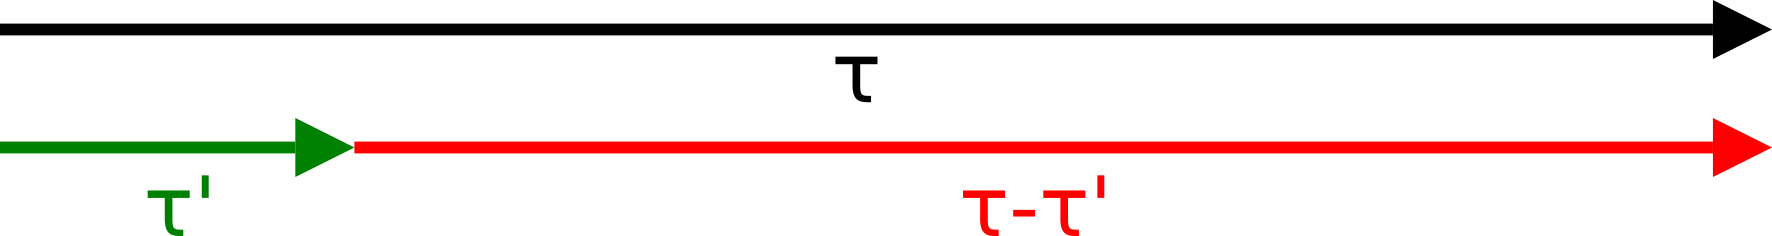
\includegraphics[width=\columnwidth]{figures/05_tau_short_long.png}
    \caption{$\tau$ value divide in short and long response.}
    \label{fig:tau_short_long}
\end{figure}

To compute the short and long response, we start redefining the returns as

\begin{align}\label{eq:short_long_return}
    r^{p}_{i}\left(t,\tau\right)&=\ln\left(\frac{m_{i}\left(t+\tau\right)}
    {m_{i} \left(t\right)}\right) \nonumber \\
    &=\ln\left(\frac{m_{i}\left(t+\tau\right)}{m_{i}\left(t+\tau'\right)}
    \cdot\frac{m_{i} \left(t+\tau'\right)}{m_{i}\left(t\right)}\right)
    \nonumber \\
    &=\ln\left(\frac{m_{i}\left(t+\tau\right)}{m_{i}\left(t+\tau'\right)}
    \right)+ \ln\left(\frac{m_{i}\left(t+\tau'\right)}{m_{i}\left(t\right)}
    \right)\nonumber \\
    &\approx\frac{m_{i}\left(t+\tau\right)-m_{i}\left(t+\tau'\right)}
    {m_{i}\left(t+\tau'\right)} +\frac{m_{i}\left(t+\tau'\right)-m_{i}
    \left(t\right)}{m_{i}\left(t\right)}
\end{align}

The second term of the right part is constant with respect to $\tau$. That
means, the main signal of the return come from the short return. The long
return does not give a significant contribution to the complete return.
Replacing Equation \ref{eq:short_long_return} in the response function we have

\begin{align}\label{eq:short_long_response}
    R^{p}_{ij}\left(\tau\right)&=\left\langle r^{p}_{i}\left(t, \tau\right)
    \cdot\varepsilon^{p}_{j}\left(t\right)\right\rangle _{p} \nonumber \\
    &\approx\left\langle \frac{m_{i}\left(t+\tau\right)-m_{i}
    \left(t+\tau'\right)} {m_{i}\left(t+\tau'\right)}\cdot\varepsilon_{j}
    \left(t\right)\right\rangle _{t\in\tau-\tau'} \nonumber \\
    & +\left\langle \frac{m_{i}
    \left(t+\tau'\right)-m_{i}\left(t\right)}{m_{i}\left(t\right)}
    \cdot\varepsilon_{j}\left(t\right)\right\rangle _{t\in\tau'}
\end{align}

Where the first term in the right side of Equation \ref{eq:short_long_response}
is the long response and the right term is the short response. Again, the right
term of Equation \ref{eq:short_long_response} is independent of $\tau$.

\begin{figure*}[htbp]
    \centering
    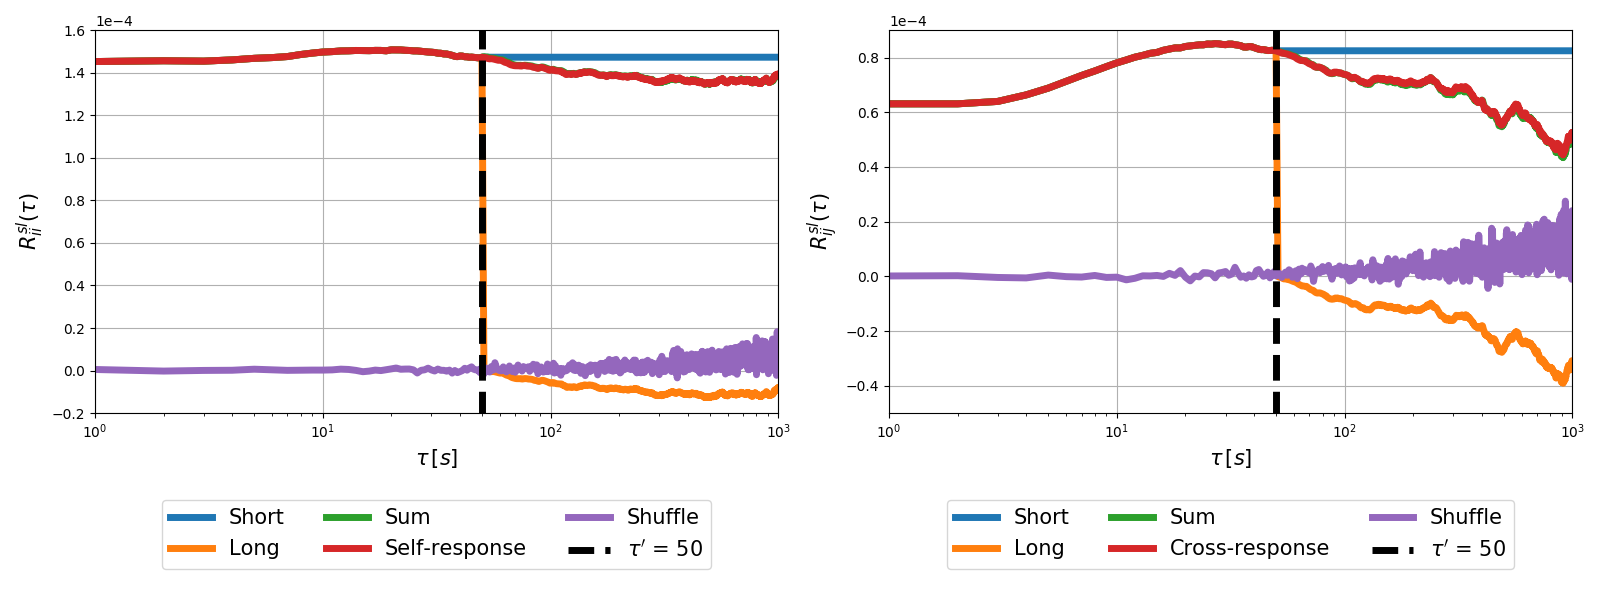
\includegraphics[width=\textwidth]
    {figures/05_short_long_AAPL_MSFT.png}
    \caption{Cross-response}
    \label{fig:short_long_cross-response}
\end{figure*}
% \caption{Self- and cross-response functions $R^{p}_{ij}\left(\tau\right)$ excluding
%          $\varepsilon^{p}_{j}\left(t\right) = 0$ in 2008 versus time lag $\tau$ on a
%          logarithmic scale using a $\tau'=40$. a) self-response function of Apple Inc. stock,
%          b) cross-response function of Apple Inc-Microsoft Corp. stocks.}
% \label{fig:short_long_responses}

\textcolor{red}{Check the legend position of the figure, change the scale to
                seconds in the axis, find a way to make more general the
                results. Maybe the average can help. Maybe repeat the analysis
                for the trade time scale.}

The results in Fig. \ref{fig:short_long_responses} show the short response, the
long response, the addition of the short response and long response (Sum), the
original response, a random response and the value of $\tau'$.

Before $\tau'$, the short response and long response are the same, as the self
and cross-response definition do not define these values for values smaller
than $\tau '$, so it is computed as the original response. After $\tau'$, the
short response is a strong constant signal. On the other hand, the long
response immediately fades, showing the small contribution to the final
response. To compare the significance of the long response, I added a random
response made with the trade signs used to compute the response but with a
shuffle order. The long response and the random response are comparable, and
show how the long response is not representative in the final response.
If we add the short and long response, we obtain the original response. In Fig.
\ref{fig:short_long_responses}, the original response (red line) has the same
shape to the addition of the short and long response (green line). I analyzed
the short and long responses with different $\tau '$ values
($10s, 20s, 30s, 40s, 50s, 60s, 70s, 80s, 90s, 100s$). On average, the maximum
response is around $\tau = 40$. That means the long response before this value
have some positive values and after this value have all negative values.